\chapter{Checking, Exporting and Delivering Traceable Figures}

Zhou, a doctoral student in materials science, finally submitted his manuscript on interfacial passivation in perovskite solar cells. Two weeks later, instead of entering peer review, the manuscript returned from the editorial office with a technical notice citing two defects. First, although Figure 2 had been uploaded as a PDF file, the publisher's preflight check flagged both the current-density--voltage ($J\text{--}V$) curves and the stability traces as low-resolution bitmaps rather than vector line art. Second, once panel \textbf{a}---the device architecture schematic---was scaled down to fit the journal's column grid, its layer labels shrank to $5\ \text{pt}$, below the journal's $7\ \text{pt}$ minimum for final printed text.

That afternoon, a collaborator who reads manuscripts on paper walked into the lab holding a black-and-white laser printout. Pointing to the two solid curves in the bottom row of Figure 2, she asked: ``In grayscale, these two traces have the exact same shade of grey---which one is the control and which one is the modified device?'' Minutes later, a junior graduate student taking over the project asked Zhou for the source files of Figure 2c to replot the data for a group-meeting slide deck. On the shared drive, she found \texttt{fig2\_final.png}, \texttt{fig2\_final2.pdf}, and \texttt{fig2\_ok\_zh.png}. Nobody could tell which file matched the submitted manuscript, where the underlying CSV table lived, or what prompts and revision instructions had produced the schematic base images.

None of these problems involved the physics of perovskite passivation, yet together they delayed peer review, obscured the experimental comparison for monochrome and colour-vision-deficient readers, and broke reproducibility inside the lab. A scientific figure is finished only when it passes a systematic \textbf{prepress technical inspection}---covering effective resolution, final font size and line weight, vector versus container structure, and colour/grayscale legibility---and is packaged into a \textbf{traceable delivery archive} that a colleague can use without asking the author a single question. This chapter turns that final check into explicit arithmetic, verifiable inspection commands, and a reusable archive structure.

\section{Physical size, pixels and effective resolution}

In submission portals and lab meetings, ``Is this figure at least 300 dpi?'' is the most frequently asked---and most frequently misunderstood---question in scientific publishing. Answering it requires separating three independent physical quantities:

\begin{enumerate}
\item \textbf{Pixel dimensions:} The horizontal and vertical grid count stored inside a bitmap file, such as $1920 \times 1080\ \text{px}$ or $2008 \times 1417\ \text{px}$. This discrete array is the only spatial information the bitmap actually holds.
\item \textbf{Physical size:} The real-world width and height at which the figure appears on a printed page or poster, measured in millimetres ($\text{mm}$) or inches ($\text{in}$, where $1\ \text{in} = 25.4\ \text{mm}$), such as a single column of $85\ \text{mm}$ or a double column of $180\ \text{mm}$ or $190\ \text{mm}$.
\item \textbf{Effective resolution:} The number of pixels allocated per inch of physical width once the bitmap is scaled to its final page dimensions, expressed in pixels per inch ($\text{ppi}$, routinely called $\text{dpi}$ in journal guidelines).
\end{enumerate}

A single geometric identity connects all three quantities (Figure~\ref{fig:ch13-01}):
\begin{gather*}
\text{Effective resolution (ppi)} = \frac{\text{Width in pixels (px)}}{\text{Physical width (mm)} \div 25.4} \\[3pt]
\text{Required pixels (px)} = \frac{\text{Physical width (mm)}}{25.4} \times \text{Target dpi}
\end{gather*}

\begin{figure}[htbp]\centering
\makebox[\linewidth][c]{% FIG ch13-01 pixels, physical size, effective resolution (English)
% Column widths are drawn at 1:2 (1 mm of column width = 0.5 mm on the page).
\begin{tikzpicture}[x=1mm, y=1mm, font=\sffamily\fontsize{8}{10}\selectfont, text=BookInk,
    >=Stealth]
  \tikzset{
    lbl/.style={inner sep=0pt, outer sep=0pt, anchor=south west},
    result/.style={inner sep=0pt, outer sep=0pt, anchor=north west},
    tick/.style={inner sep=0.4pt, outer sep=0pt, anchor=north},
    takeaway/.style={draw=BookTeal, line width=0.6pt, fill=white, rounded corners=1.2pt,
      inner sep=1.8mm, align=center, text width=122mm, font=\sffamily\fontsize{8}{10.5}\selectfont},
  }

  % One bitmap file
  \draw[BookRule, line width=0.6pt, fill=BookPale, rounded corners=1.2pt]
    (0.6, 43.0) rectangle (30.0, 76.8);
  \begin{scope}
    \clip (6.2, 63.2) rectangle (24.2, 73.325);
    \fill[white] (6.2, 63.2) rectangle (24.2, 73.325);
    \foreach \i in {0,...,15} {
      \foreach \j in {0,...,8} {
        \pgfmathparse{mod(\i+\j,2) ? 18 : 8}
        \fill[BookTeal!\pgfmathresult]
          (6.2+1.125*\i, 63.2+1.125*\j) rectangle ++(1.125, 1.125);
      }
    }
  \end{scope}
  \draw[BookRule, line width=0.4pt] (6.2, 63.2) rectangle (24.2, 73.325);
  \node[align=center, inner sep=0pt, anchor=center] at (15.3, 53.2)
    {{\fontsize{9}{11}\selectfont File:}\\[2.5pt]1920 × 1080\,px};

  % Shared origin of the two width bars. 85 mm -> 42.5 mm; 180 mm -> 90 mm.
  \def\xO{36.2}
  \def\sS{0.5}

  \node[lbl] at (\xO, 73.4) {Single column 85\,mm};
  \fill[BookTeal] (\xO, 68.4) rectangle ({\xO+85*\sS}, 71.8);
  \node[result] at (\xO, 66.6) {1920 ÷ (85 ÷ 25.4) ≈ \textbf{574\,ppi}};

  \node[lbl] at (\xO, 56.6) {Double column 180\,mm};
  \fill[BookTeal] (\xO, 51.6) rectangle ({\xO+180*\sS}, 55.0);
  \node[result] at (\xO, 49.8) {1920 ÷ (180 ÷ 25.4) ≈ \textbf{271\,ppi}};

  \draw[BookInk, line width=0.55pt, ->] (30.0, 70.1) -- (\xO, 70.1);
  \draw[BookInk, line width=0.55pt, ->] (30.0, 53.3) -- (\xO, 53.3);

  % Ruler in the same scale as the bars
  \draw[BookInk, line width=0.7pt] (\xO, 41.2) -- ({\xO+180*\sS}, 41.2);
  \foreach \mm/\lab in {0/0, 85/85, 180/180\,mm} {
    \draw[BookInk, line width=0.55pt] ({\xO+\mm*\sS}, 41.2) -- ({\xO+\mm*\sS}, 39.6);
    \node[tick] at ({\xO+\mm*\sS}, 39.3) {\lab};
  }
  \node[inner sep=0pt, outer sep=0pt, anchor=north west] at (0.6, 34.6)
    {Same scale (1\,mm of column width = 0.5\,mm on this page)};

  \node[takeaway, anchor=north west] at (0.6, 29.2) {%
    effective ppi = pixels ÷ (width in mm ÷ 25.4)\\[2pt]
    Changing the dpi tag does not change the pixel count.};
\end{tikzpicture}
}
\caption{The same file at two widths has two effective resolutions. Effective resolution depends on pixel count and final printed width, not on the dpi tag stored in the file.}\label{fig:ch13-01}
\end{figure}

Writing down this ratio dispels two common misconceptions immediately.

The first misconception is \textbf{mistaking the metadata dpi tag in a file header for effective resolution}. PNG, TIFF, and JPEG headers store a nominal density number---often $72\ \text{dpi}$ or $96\ \text{dpi}$ by default. If you open an image in an editor, uncheck ``Resample,'' and change that header field from $72$ to $300$, not a single pixel is added. When a layout engine stretches that file across a double column, it still blurs if the pixel count is too low. Conversely, a file tagged $72\ \text{dpi}$ that measures $2126\ \text{px}$ across delivers a genuine $300\ \text{ppi}$ across a $180\ \text{mm}$ double column.

The second misconception is \textbf{discussing resolution without naming the target layout width}. As Figure~\ref{fig:ch13-01} shows, placing a $1920 \times 1080\ \text{px}$ bitmap into an $85\ \text{mm}$ single column ($3.35\ \text{in}$) gives $1920 \div (85 \div 25.4) \approx 574\ \text{ppi}$, satisfying most requirements for photographs and combination art. Stretching that exact same file across a $180\ \text{mm}$ double column ($7.09\ \text{in}$) drops its effective resolution to $1920 \div (180 \div 25.4) \approx 271\ \text{ppi}$---below the $300\ \text{dpi}$ baseline even for photographs. Similarly, a $1024\ \text{px}$-wide image yields $306\ \text{ppi}$ at $85\ \text{mm}$ single-column width, but only $144\ \text{ppi}$ at $180\ \text{mm}$ double-column width, producing visible staircase aliasing.

Table~\ref{tab:ch13-px-calc} summarizes the conversions between standard journal column widths, required pixel counts, and effective resolution. Checking this arithmetic takes ten seconds before you create a canvas or export a file.

\begin{table}[htbp]\centering\footnotesize
\setlength{\tabcolsep}{4pt}
\renewcommand{\arraystretch}{1.18}
\caption{Converting between target layout widths, required pixel counts, and effective resolution.}\label{tab:ch13-px-calc}
\begin{tabularx}{\linewidth}{@{}>{\raggedright\arraybackslash}p{28mm}>{\raggedright\arraybackslash}p{28mm}>{\raggedright\arraybackslash}p{28mm}Y@{}}
\toprule
\textbf{Direction} & \textbf{Layout or file parameter} & \textbf{Target condition} & \textbf{Arithmetic and result} \\
\midrule
Width \& dpi $\rightarrow$ pixels & Single column $85\ \text{mm}$ ($3.35\ \text{in}$) & Photo $300\ \text{dpi}$ / combo $600\ \text{dpi}$ & $85 \div 25.4 \times 300 \approx 1004\ \text{px}$; $\times 600 \approx 2008\ \text{px}$ \\
Width \& dpi $\rightarrow$ pixels & Double column $180\ \text{mm}$ ($7.09\ \text{in}$) & Photo $300\ \text{dpi}$ / combo $600\ \text{dpi}$ & $180 \div 25.4 \times 300 \approx 2126\ \text{px}$; $\times 600 \approx 4252\ \text{px}$ \\
Width \& dpi $\rightarrow$ pixels & Double column $190\ \text{mm}$ ($7.48\ \text{in}$) & Elsevier line art $1000\ \text{dpi}$ & $190 \div 25.4 \times 1000 \approx 7480\ \text{px}$ (combo $500\ \text{dpi} \approx 3740\ \text{px}$) \\
Pixels \& width $\rightarrow$ ppi & $1920\ \text{px}$-wide file & At $85\ \text{mm}$ single / $180\ \text{mm}$ double & Single: $1920 \div 3.35 \approx 574\ \text{ppi}$; double: $1920 \div 7.09 \approx 271\ \text{ppi}$ \\
Pixels \& width $\rightarrow$ ppi & $1024\ \text{px}$-wide file & At $85\ \text{mm}$ single / $180\ \text{mm}$ double & Single: $1024 \div 3.35 \approx 306\ \text{ppi}$; double: $1024 \div 7.09 \approx 144\ \text{ppi}$ \\
\bottomrule
\end{tabularx}
\end{table}

When a bitmap has too few pixels, many authors try to enlarge it by mathematical interpolation (`upsampling'). Figure~\ref{fig:ch13-02} uses the simulated perovskite $J\text{--}V$ curve from our case ($85 \times 60\ \text{mm}$) to compare a $150\ \text{dpi}$ render enlarged $4\times$ by bicubic interpolation against a plot rendered directly at $600\ \text{dpi}$.

\begin{figure}[htbp]\centering
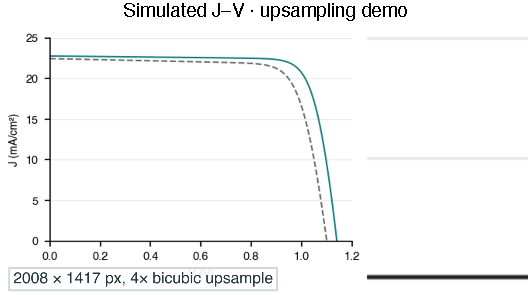
\includegraphics[width=85mm]{figures/ch13/ch13-02a-upsampled-en.pdf}\\[1.5mm]
{\footnotesize (a) Rendered at $150\ \text{dpi}$ ($502 \times 354\ \text{px}$), then enlarged $4\times$ by bicubic interpolation to $2008 \times 1417\ \text{px}$}\\[3mm]
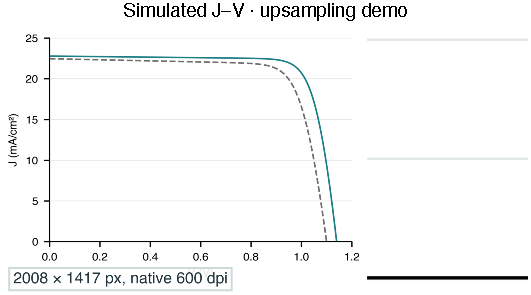
\includegraphics[width=85mm]{figures/ch13/ch13-02b-native-en.pdf}\\[1.5mm]
{\footnotesize (b) Rendered directly at $600\ \text{dpi}$ ($2008 \times 1417\ \text{px}$)}
\caption{Same pixel count, different information. (a) Rendered at 150 dpi, then interpolated to 600 dpi; (b) rendered directly at 600 dpi. Insets are magnified 8$\times$. Simulated data.}\label{fig:ch13-02}
\end{figure}

Compare the two panels of Figure~\ref{fig:ch13-02}. Both files measure $2008 \times 1417\ \text{px}$, so an automated dimension check reports $600\ \text{ppi}$ for both. Yet the visual difference is unmistakable. In the full plot on the left of Figure~\ref{fig:ch13-02}a, the tick numerals (\texttt{0.0}--\texttt{1.2} and \texttt{0}--\texttt{25}), vertical axis title (`\texttt{J (mA/cm\textsuperscript{2})}'), and curves look blurry. On the right, the $8\times$ inset crops the bottom black axis spine and two light-grey horizontal grid lines: in Figure~\ref{fig:ch13-02}a, both the axis spine and grid lines carry fuzzy grey halos along their upper and lower edges---the smear left behind when a $502 \times 354\ \text{px}$ grid is interpolated $4\times$. In Figure~\ref{fig:ch13-02}b, rendered directly at $600\ \text{dpi}$, every character and line edge stays crisp.

Notice also two layout flaws inside Figure~\ref{fig:ch13-02} itself: first, the bottom-left pixel-count box was placed at a fixed relative coordinate and overlaps the top half of the horizontal axis title `\texttt{V (V)}'; second, the vertical crop window for the $8\times$ inset captured only the flat grid lines and bottom axis rather than the curved $J\text{--}V$ knee and tick text. When you run an $800\%$ zoom check on your own figures, always pan across curve knees, diagonal strokes, and superscripts rather than inspecting only flat horizontal lines.

Mathematical interpolation (bilinear, bicubic, or Lanczos) fills smooth intermediate values between old pixels; \textbf{it increases file size without adding real spatial information}. Even more hazardous is \textbf{generative AI super-resolution upscaling}. Passing a low-resolution scanning electron micrograph (SEM), fluorescence image, or Western blot through an AI upscaler produces sharp-looking edges by hallucinating textures from its training corpus---turning blurry grain boundaries into crisp facets or inventing pores in background noise. As Chapter 8 established, primary experimental images are observational evidence: \textbf{never apply generative AI upscaling or redrawing to scientific evidence images}. If an experimental panel lacks effective resolution, either re-export the full-resolution master from the instrument or reduce that panel's physical millimetre width in the layout and document its native pixel count in the processing log.

In \scidraw{}, distinguish between two export mechanisms: general image-conversion utilities map nominal dpi choices to fixed maximum pixel side lengths and may invoke AI upscaling when a source image is small, so they must never be used to ``boost dpi'' on experimental micrographs; by contrast, the multi-panel assembly workspace (\sdtool{multi-panel-figure-maker}) calculates canvas dimensions strictly from target physical millimetres and dpi, recording each panel's native pixels, physical width, and effective resolution in \texttt{processing-log}.

\section{Text and line weight at final size}

The second frequent cause of technical returns and reader frustration is \textbf{unintended shrinkage of font sizes and line weights at final print width}.

Many researchers draft plots in Python (Matplotlib), R, Origin, or PowerPoint on a wide default canvas while looking at a large monitor: $10\ \text{pt}$ axis labels look clear on screen, but shrink to near-illegibility when scaled into a narrow journal column. Whenever a wide canvas is scaled down to a narrower target column width, every font size and stroke width scales down by the exact same linear ratio:
\[
\text{Final font size (pt)} = \text{Drafting font size (pt)} \times \frac{\text{Final layout width (mm)}}{\text{Drafting canvas width (mm)}}
\]

Two everyday scenarios show how fast text drops below journal limits:
\begin{itemize}
\item \textbf{Scaling down a wide Matplotlib canvas:} The paired-comparison plot from Chapters 1 and 5 was originally drafted on a $7.3\ \text{in}$ ($185.4\ \text{mm}$) canvas with $10\ \text{pt}$ text. Across a $180\ \text{mm}$ double column, the text prints at $10 \times 180 \div 185.4 \approx 9.7\ \text{pt}$. Placed into an $85\ \text{mm}$ single column (or half of a double-column composite), however, the scaling ratio becomes $85 \div 185.4 \approx 0.458$, shrinking $10\ \text{pt}$ text to $10 \times 85 \div 185.4 \approx 4.6\ \text{pt}$ ($4.58\ \text{pt}$). That falls below Elsevier's $7\ \text{pt}$ target, PLOS ONE's $8\ \text{pt}$ minimum, and even Nature's $5\ \text{pt}$ floor.
\item \textbf{Scaling down a widescreen PowerPoint slide:} A standard 16:9 slide is $33.867\ \text{cm}$ ($338.7\ \text{mm}$) wide. Shrinking a full-slide diagram into an $85\ \text{mm}$ single column scales everything by $85 \div 338.7 \approx 0.251$: $24\ \text{pt}$ headings drop to $6.0\ \text{pt}$, and $18\ \text{pt}$ notes collapse to $4.5\ \text{pt}$.
\end{itemize}

Figure~\ref{fig:ch13-03} prints both approaches for the paired-comparison dataset (8 simulated subjects, where \texttt{SIM04} drops from 18 to 17) at \textbf{actual $85\ \text{mm}$ physical width}, letting you compare $4.6\ \text{pt}$ and $7\ \text{pt}$ directly on the page.

\begin{figure}[htbp]\centering
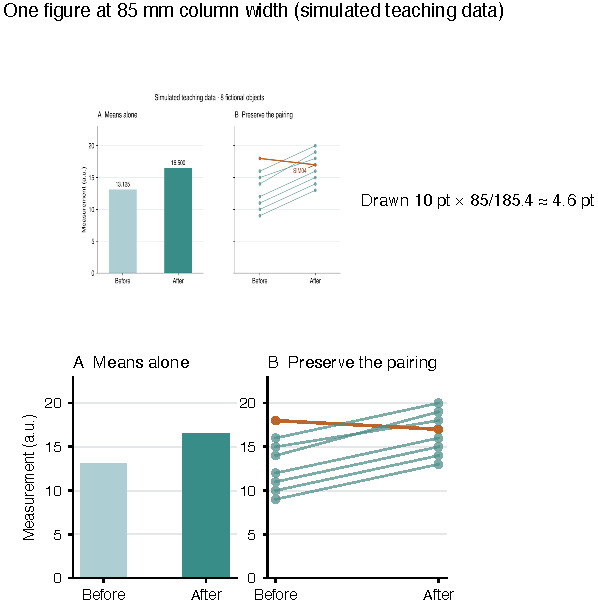
\includegraphics[width=85mm]{figures/ch13/ch13-03-text-at-final-width-en.pdf}
\caption{One figure, two outcomes in an 85 mm column. Top: drawn 7.3 in (185 mm) wide with 10 pt text, which shrinks to about 4.6 pt; bottom: drawn at final width with 7 pt text. Both are printed at actual size. Simulated teaching data.}\label{fig:ch13-03}
\end{figure}

In the top half of Figure~\ref{fig:ch13-03}, shrinking the $185.4\ \text{mm}$ plot into the single-column width reduces the vertical axis title (`\texttt{Measurement (a.u.)}'), bar-top means (`\texttt{13.125}', `\texttt{16.500}'), and subject label `\texttt{SIM04}' to about $4.6\ \text{pt}$, while thinning the axis spines and grid lines until they look faint. In the bottom half, the script set the canvas width directly to $85\ \text{mm}$, with $7\ \text{pt}$ ticks and axis labels, $8\ \text{pt}$ subplot titles (`\texttt{A Means alone}', `\texttt{B Preserve the pairing}'), $0.75\ \text{pt}$ paired lines, $1.2\ \text{pt}$ for \texttt{SIM04}, and no cluttered three-decimal bar labels. Every label reads cleanly.

Figure~\ref{fig:ch13-03} also illustrates a real layering pitfall from script assembly: the script placed a margin note at $x = 0.76$ in both rows---`\texttt{Drawn 10 pt $\times$ 85/185.4 $\approx$ 4.6 pt}' in the top row and `\texttt{Final 7 pt}' in the bottom row. Because the bottom row's two subplots span the full $85\ \text{mm}$ width out to $x = 0.98$, their white subplot canvas covered up the `\texttt{Final 7 pt}' note underneath. Always inspect the rendered page visually after combining subplots or overlays.

Line weights scale by the same ratio: a $0.5\ \text{pt}$ line on a $185\ \text{mm}$ canvas thins to $0.23\ \text{pt}$ at $85\ \text{mm}$ width, approaching the lower limit of journal rules (Elsevier specifies $0.10\text{--}1.5\ \text{pt}$) and risking broken hairlines in print.

Two habits prevent font and line-weight shrinkage:
\begin{enumerate}
\item \textbf{Set the canvas to final millimetre dimensions from the start (scale factor 1.0):} Use $\texttt{figsize}=(85/25.4,\ H/25.4)$ (or $89\ \text{mm}$ / $90\ \text{mm}$) for single-column plots and $(174/25.4,\ H/25.4)$ (or $183\ \text{mm}$ / $190\ \text{mm}$) for double-column plots so that $7\ \text{pt}$ in code prints as $7\ \text{pt}$ on paper.
\item \textbf{Print a 100\% paper proof and measure with a ruler:} Place the figure at its target millimetre width on an A4/Letter page, print at 100\% scale, check the frame width with a ruler, and measure uppercase letter height. Since $1\ \text{pt} = 1/72\ \text{in} \approx 0.353\ \text{mm}$ and sans-serif uppercase cap height is about $0.7\times$ point size, final $7\ \text{pt}$ capitals measure roughly $1.7\text{--}1.8\ \text{mm}$ tall ($8\ \text{pt} \approx 2.0\ \text{mm}$). If capitals measure under $1.2\ \text{mm}$, an unintended rescaling step occurred.
\end{enumerate}

\section{Vector, raster and container formats}

Why did the journal's preflight system reject Zhou's Figure 2 PDF as a ``low-resolution bitmap''? Because he equated a \textbf{file extension} with \textbf{what is stored inside the file}.

Graphics files fall into three structural categories (Figure~\ref{fig:ch13-04}):
\begin{itemize}
\item \textbf{Pure raster files (PNG, TIFF, JPEG):} Store a 2D pixel grid. At $800\%$ zoom, curves and letters break into square pixels. Raster formats suit photographs, micrographs, gels, and text-free generated base illustrations.
\item \textbf{True vector content (PDF, SVG, or EPS with paths and live text):} Store mathematical coordinates for lines, B\'{e}zier curves, fills, and character strings linked to embedded fonts. Edges remain sharp at any magnification, and axis labels can be selected as live text.
\item \textbf{``Container'' files (PDF, SVG, EPS, or PPTX wrapping a bitmap):} PDF, SVG, EPS, and PPTX are \textbf{compound containers}. They can hold vector paths and fonts, or they can simply wrap a single PNG/JPEG bitmap. Saving a $150\ \text{dpi}$ PNG as a PDF produces a \texttt{.pdf} file whose content is still a $150\ \text{ppi}$ bitmap.
\end{itemize}

\begin{figure}[htbp]\centering
\resizebox{\linewidth}{!}{% FIG ch13-04 what's inside the file (English)
\usetikzlibrary{arrows.meta,positioning,fit}
\begin{tikzpicture}[
  font=\sffamily\footnotesize, text=BookInk,
  card/.style={draw=BookRule, line width=0.6pt, rounded corners=3pt,
    fill=BookPale!30, minimum width=42mm, minimum height=38mm, align=center, inner sep=5pt},
]
  \node[card] (C1) at (0,0) {%
    \textbf{Raster files}\\PNG, TIFF, JPEG\\[4pt]
    \tikz{\foreach \x in {0,1,2,3} \foreach \y in {0,1,2,3}
      \fill[BookTeal!35] (\x*0.35,\y*0.35) rectangle ++(0.32,0.32);}\\[3pt]
    \scriptsize Zoom in to see pixels;\\photos and micrographs};
  \node[card, right=6mm of C1] (C2) {%
    \textbf{Vector content}\\paths and text inside PDF/SVG/EPS\\[4pt]
    \tikz{\draw[BookTeal, line width=0.8pt] (0,0.6) .. controls (0.5,1.2) and (1.2,0.2) .. (1.6,0.8);
      \node[font=\sffamily] at (0.8,0.2) {Aa};}\\[3pt]
    \scriptsize Edges stay sharp;\\selectable text, embedded fonts};
  \node[card, right=6mm of C2] (C3) {%
    \textbf{Container}\\vector-like name, bitmap inside\\[4pt]
    \tikz{\draw[BookRule, fill=white] (-0.1,-0.1) rectangle (1.7,1.3);
      \foreach \x in {0,1,2} \foreach \y in {0,1,2}
        \fill[BookInk!25] (0.2+\x*0.35,0.2+\y*0.28) rectangle ++(0.3,0.24);}\\[3pt]
    \scriptsize PDF/SVG/EPS/PPTX\\may wrap a single bitmap};

  \node[draw=BookTeal, fill=white, rounded corners=2pt, inner sep=5pt,
    text width=132mm, align=left, font=\scriptsize, below=8mm of C2] (how) {%
    \textbf{How to check:}\ 
    \texttt{pdffonts}, \texttt{pdfimages -list}, 800\,\% zoom,
    search SVG for \texttt{<image}, unzip PPTX \texttt{ppt/media/}.};

  \node[draw=BookRule, fill=BookPale!15, rounded corners=2pt, inner sep=4pt,
    text width=132mm, align=left, font=\scriptsize, below=3mm of how] {%
    \textbf{SciDraw AI exports to note:}
    declarative chart PDF/EPS is raster-wrapped;
    image-to-SVG text mode keeps a bitmap background;
    image-to-PPTX is background + OCR boxes;
    multi-panel PPTX uses bitmap panels and text labels.};
\end{tikzpicture}
}
\caption{The file extension does not tell you what is inside. PDF, SVG, EPS and PPTX can hold vector objects or just wrap a bitmap.}\label{fig:ch13-04}
\end{figure}

Five practical checks reveal whether a container holds true vector objects or a wrapped bitmap:

\begin{enumerate}
\item \textbf{Check embedded fonts with \texttt{pdffonts} (command line):} The Poppler utility \texttt{pdffonts} lists all fonts in a PDF and whether they are embedded (\texttt{emb=yes}) and subsetted (\texttt{sub=yes}). If a figure displays visible text yet \texttt{pdffonts} outputs nothing, the text has either been rasterized into pixels or converted into uneditable outline paths. Note that journals such as Nature explicitly instruct authors neither to rasterize line art/text nor to outline text.
\item \textbf{List internal bitmaps with \texttt{pdfimages -list} (command line):} This command reports every raster image inside a PDF, including pixel dimensions, colour space, and effective \texttt{x-ppi}/\texttt{y-ppi}. If a standalone line chart appears as a full-page bitmap in \texttt{pdfimages -list}, it is a raster container. Conversely, in a multi-panel PDF like Chapter 9's Figure 2 (schematic bitmaps in \textbf{a}, \textbf{b}; data plots in \textbf{c}, \textbf{d}), \texttt{pdfimages -list} \textbf{should list only panels a and b}, while panels \textbf{c} and \textbf{d} stay pure vector. Photographs and generated bases are naturally raster; plotted curves and text must stay vector.
\item \textbf{Zoom to 800\% and select text in a PDF viewer (no command line):} Try highlighting axis labels with the text cursor, then zoom to $800\%$ to see whether curves stay smooth or break into pixel stairs (or use Adobe Acrobat Pro's ``Preflight'' object inspector).
\item \textbf{Search SVG files in a text editor:} Open the \texttt{.svg} file and search for \texttt{<image}. A file containing only a Base64 PNG string is a bitmap wrapper; a true vector SVG contains hundreds of \texttt{<path>}, \texttt{<line>}, and \texttt{<text>} tags.
\item \textbf{Unzip PPTX files:} Copy \texttt{.pptx} to \texttt{.zip}, extract it, and inspect \texttt{ppt/media/} to see every embedded bitmap.
\end{enumerate}

Figure~\ref{fig:ch13-05} and Table~\ref{tab:ch13-02} compare a true vector PDF (\texttt{vector.pdf}, with \texttt{pdf.fonttype = 42}) and a $150\ \text{ppi}$ bitmap-container PDF (\texttt{container.pdf}) generated from the same simulated perovskite $J\text{--}V$ data\allowbreak{} ($85 \times 60\ \text{mm}$).

\begin{figure}[htbp]\centering
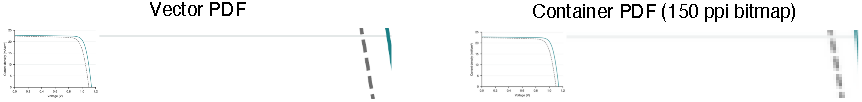
\includegraphics[width=\linewidth]{figures/ch13/ch13-05-vector-vs-container-en.pdf}
\caption{Both are PDFs. Left: vector paths and embedded fonts stay sharp when magnified; right: a wrapped 150 ppi bitmap shows its pixels. Simulated data.}\label{fig:ch13-05}
\end{figure}

\begin{table}[htbp]\centering\footnotesize
\setlength{\tabcolsep}{4pt}
\renewcommand{\arraystretch}{1.18}
\caption{Measured output from running \texttt{pdffonts} and \texttt{pdfimages -list} on the two PDF files in Figure~\ref{fig:ch13-05}.}\label{tab:ch13-02}
\begin{tabularx}{\linewidth}{@{}>{\raggedright\arraybackslash}p{26mm}>{\raggedright\arraybackslash}p{23mm}Y@{}}
\toprule
\textbf{File and nature} & \textbf{Command} & \textbf{Measured output summary and interpretation} \\
\midrule
\texttt{vector.pdf} (true vector PDF) & \texttt{pdffonts} & Lists \texttt{Helvetica} (\texttt{CID TrueType}) with \texttt{emb=yes}, \texttt{sub=yes} (plus \texttt{FandolHei-Regular} in the Chinese build), confirming embedded font subsets \\
\texttt{vector.pdf} (true vector PDF) & \texttt{pdfimages -list} & No entries (empty output), proving axes, grid lines, and both curves are pure vector paths \\
\texttt{container.pdf} (bitmap container) & \texttt{pdffonts} & No entries (empty output), proving visible axis labels are no longer text objects \\
\texttt{container.pdf} (bitmap container) & \texttt{pdfimages -list} & Lists 1 RGB bitmap on page 1 ($502 \times 355\ \text{px}$, \texttt{x-ppi=150} when wrapped directly; or degraded to $260 \times 182\ \text{px}$, \texttt{x-ppi=100} if re-saved via Matplotlib \texttt{imshow} at default \texttt{savefig.dpi=100}) \\
\bottomrule
\end{tabularx}
\end{table}

Alongside the sharp vector inset on the left and the pixelated bitmap inset on the right of Figure~\ref{fig:ch13-05}, this test highlights two subtle traps in real workflows:

First is the \textbf{missing-glyph trap in embedded fonts}. In Figure~\ref{fig:ch13-05}, the English y-axis label `\texttt{Current density (mA/cm\textsuperscript{2})}' uses Helvetica, which contains the Unicode superscript two (`\texttt{\textsuperscript{2}}', \texttt{U+00B2}). When the same script assigns the entire label to a font lacking \texttt{U+00B2}---as occurred in the Chinese build with \texttt{FandolHei-Regular.otf}, or when a specialty font lacks $\mu$ or minus signs---\texttt{pdffonts} still reports \texttt{emb=yes}, yet the superscript silently disappears into a blank space in the vector PDF and turns into a missing-glyph box (`tofu') in the container PDF. Always pair \texttt{pdffonts} with an $800\%$ visual check, and render scientific units via math mode (\texttt{\$\textbackslash mathrm\{mA\textbackslash,cm\textasciicircum\{-2\}\}\$}) or a verified Latin/symbol font.

Second is \textbf{silent downsampling during secondary wrapping}. As noted in Table~\ref{tab:ch13-02}, placing a $150\ \text{dpi}$ bitmap ($502 \times 354\ \text{px}$) into a new Matplotlib figure via \texttt{imshow} and calling \texttt{savefig("container.pdf")} without a \texttt{dpi} argument resamples the image at the default \texttt{savefig.dpi = 100}, shrinking it to $260 \times 182\ \text{px}$ ($100\ \text{ppi}$). Running \texttt{pdfimages -list} catches this immediately.

Keep in mind the actual internal structure of exports from current \scidraw{} modules:
\begin{itemize}
\item \textbf{Scientific visualization (\sdtool{sci-vis}):} PDF and EPS files exported from its declarative chart pathway are \textbf{raster-wrapped containers}. When a journal requires true vector data plots with embedded fonts, download the verified data table from \sdtool{sci-vis} and run a deterministic script (\texttt{pdf.fonttype = 42}) at final physical dimensions.
\item \textbf{Image-to-SVG and image-to-PPTX:} Converting a bitmap to SVG in text-layer mode retains a bitmap background underneath; converting to PPTX yields a background bitmap plus OCR text boxes rather than semantic vector objects.
\item \textbf{Multi-panel assembly (\sdtool{multi-panel-figure-maker}):} In exported PPTX files, panels are bitmaps and panel letters (\textbf{a}--\textbf{d}) are editable text boxes; curves inside panels cannot be ungrouped in PowerPoint.
\end{itemize}

\section{Colour: RGB/CMYK, grayscale and colour-vision deficiency}

Colour inspection answers three questions: Which colour space should you submit? Can groups be told apart in black-and-white printouts? And does the figure work for readers with colour-vision deficiency (CVD)?

\subsection*{RGB versus CMYK: keep an sRGB master and do not convert blindly}

Screens mix red, green, and blue light (additive RGB, wide gamut), whereas printing presses layer cyan, magenta, yellow, and black inks (subtractive CMYK, narrower gamut, especially in bright greens and cyans).

Older tutorials often advised converting all figures to CMYK before submission. Today, most scientific reading happens online in HTML and PDF, and the three official publisher guidelines verified for this chapter (as of 29 October 2026) all recommend or accept RGB:
\begin{itemize}
\item \textbf{Nature:} Recommends submitting RGB artwork; production converts RGB to CMYK for print while keeping vivid RGB originals in online HTML and PDF editions.
\item \textbf{Elsevier:} Explicitly states ``RGB preferred.''
\item \textbf{PLOS ONE:} Requires $8\ \text{bit}$/channel RGB or grayscale.
\end{itemize}

Converting to CMYK locally with an arbitrary ICC profile dulls colours for online readers and risks a second colour shift on press. \textbf{Always retain and submit an RGB master with an embedded sRGB profile; convert a copy to CMYK only when a journal explicitly mandates it, and inspect saturated hues after conversion.}

\subsection*{Grayscale legibility: check perceptual lightness $L^*$, not the RGB average}

When Zhou's collaborator asked which curve was the control on her monochrome printout, she uncovered a real issue left in our Chapter 9 and Chapter 12 drafts.

In Chapter 12, we paired dark grey (\texttt{\#6E6E6E}, control) with deep teal (\texttt{\#1B7F86}, modified). On a colour monitor, their perceptual colour difference (CAM02-UCS $\Delta E$) is $19.8$. In grayscale, however, human brightness perception does not average $(R + G + B)/3$; it follows spectral sensitivity captured by \textbf{relative luminance ($Y$) and CIE 1976 perceptual lightness ($L^*$)}. After linearizing gamma-encoded sRGB channels into $(R_{\text{lin}}, G_{\text{lin}}, B_{\text{lin}})$, Rec.~709 luminance is:
\[
Y = 0.2126\,R_{\text{lin}} + 0.7152\,G_{\text{lin}} + 0.0722\,B_{\text{lin}}
\]
Mapping $Y$ to CIE $L^* \in [0, 100]$ for our case colours yields:
\begin{itemize}
\item Control dark grey \texttt{\#6E6E6E} ($\text{RGB} = 110, 110, 110$): \textbf{$L^* = 46.4$};
\item Modified deep teal \texttt{\#1B7F86} ($\text{RGB} = 27, 127, 134$): because red is near zero, \textbf{$L^* = 48.4$};
\item Draft red \texttt{\#CC0000} ($\text{RGB} = 204, 0, 0$): $L^* = 42.5$;
\item Draft green \texttt{\#2CA02C} ($\text{RGB} = 44, 160, 44$): $L^* = 57.9$.
\end{itemize}

The calculation explains the printout failure immediately: \textbf{control grey ($L^* = 46.4$) and modified teal ($L^* = 48.4$) differ by only $2.0$ lightness units, collapsing their grayscale difference to $\Delta E = 2.1$!} Two solid lines at $L^* = 46.4$ and $48.4$ look identical on paper. Every figure needs a true $L^*$ grayscale check.

\subsection*{Colour-vision deficiency simulation and redundant encoding}

Human trichromatic vision uses long- ($L$, red-sensitive), middle- ($M$, green-sensitive), and short-wavelength ($S$, blue-sensitive) retinal cones. Inherited CVD falls into three classes:
\begin{enumerate}
\item \textbf{Protan ($L$-cone alteration):} Protanomaly and protanopia; reds and greens confuse, and pure reds appear darkened.
\item \textbf{Deutan ($M$-cone alteration):} Deuteranomaly and deuteranopia; the most common type, collapsing reds and greens into similar olive-brown tones.
\item \textbf{Tritan ($S$-cone alteration):} Tritanomaly and tritanopia; rarer, affecting blue--green and yellow--violet pairs.
\end{enumerate}

As Wong (2011) noted, roughly $8\%$ of men (and about $0.5\%$ of women) of Northern European ancestry have red--green CVD. Crameri, Shephard, and Heron (2020) further showed that rainbow colormaps (such as Jet) both fail CVD readers and distort data gradients due to uneven $L^*$ profiles.

To simulate CVD computationally, Brettel, Vi\'{e}not, and Mollon (1997) projected colours in LMS cone space for dichromacy, while Machado, Oliveira, and Fernandes (2009) modelled spectral shifts across severities $0\text{--}100$ using $3 \times 3$ matrices in \textbf{linear RGB space}. Figure~\ref{fig:ch13-06} applies the Machado et al.\ (2009) model at $\text{severity} = 100$ (via \texttt{colorspacious} v1.1.2, verified against the original paper's matrices) across three palette rows and five views, printing the CAM02-UCS $\Delta E$ between the two curves in the upper-right corner of each cell.

\begin{figure}[htbp]\centering
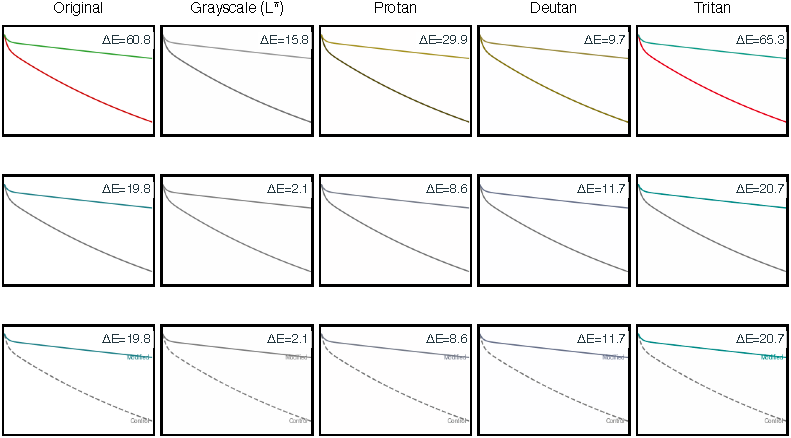
\includegraphics[width=\linewidth]{figures/ch13/ch13-06-grayscale-and-cvd-en.pdf}
\caption{Three colour schemes for one plot, seen in grayscale and under simulated colour-vision deficiencies. Row 2 (the Chapter 12 colours) is almost indistinguishable in grayscale; row 3 adds a line style and stays distinguishable in every view. Simulations use the Machado et al. (2009) model at full severity and are approximations. Simulated data.}\label{fig:ch13-06}
\end{figure}

Inspecting Figure~\ref{fig:ch13-06} row by row shows:
\begin{itemize}
\item \textbf{Row 1 (solid red \texttt{\#CC0000} and solid green \texttt{\#2CA02C}):} Strong contrast in Original ($\Delta E = 60.8$) and Tritan ($\Delta E = 65.3$), and moderate grayscale separation ($\Delta E = 15.8$ from $L^* = 42.5$ vs.\ $57.9$), but under Deutan (column 4) both curves become murky olive-brown ($\Delta E = 9.7$), inviting mix-ups when matched against a legend box.
\item \textbf{Row 2 (Chapter 12 initial palette: solid grey \texttt{\#6E6E6E} and solid teal \texttt{\#1B7F86}):} Preserves chromatic contrast in Protan ($\Delta E = 8.6$), Deutan ($\Delta E = 11.7$), and Tritan ($\Delta E = 20.7$), but collapses in CIE $L^*$ Grayscale (column 2) to \textbf{$\Delta E = 2.1$}.
\item \textbf{Row 3 (revised: dashed grey \texttt{\#6E6E6E} control, solid teal \texttt{\#1B7F86} modified, plus direct labels `\texttt{Modified}' and `\texttt{Control}'):} The colour $\Delta E$ values ($19.8$, $2.1$, $8.6$, $11.7$, $20.7$) are identical to Row 2 because the hex colours did not change, yet adding \textbf{line style (dashed vs.\ solid)} and \textbf{direct endpoint labels} makes the two groups instantly distinguishable across all five columns.
\end{itemize}

Notice one typographic detail in Row 3 of Figure~\ref{fig:ch13-06}: in these small thumbnails, the $5\ \text{pt}$ labels `\texttt{Modified}' and `\texttt{Control}' were vertically centred right on the $t = 980\ \text{h}$ curve endpoints, so the curve strokes pass through the middle of the words. In full-sized publication finals, offset direct labels slightly above, below, or beside the curve end so lines never strike through text.

Remember two limits of CVD simulations: first, simulations are mathematical approximations for a standard display and observer, not an absolute certification; second, as Machado et al.\ (2009) noted, empirical data for tritan defects are sparser, making tritan simulation less reliable than protan/deutan. The robust solution is \textbf{redundant encoding}: always combine colour with distinct line styles, marker shapes, or direct labels.

\section{Technical checks with \sdtool{figure-checker}}

You can automate bitmap preflight checks using the figure checker in \scidraw{} (\sdtool{figure-checker}). Upload a PNG, JPEG, WebP, or TIFF, select the \textbf{figure type} (\textit{Photograph}, \textit{Combination}, or \textit{Line art}), and choose the \textbf{target layout width} (preset $85\ \text{mm}$ single column, $180\ \text{mm}$ double column, or \textit{Custom width} in millimetres). The tool reports six items with visual previews: (1) \textbf{effective resolution} ($\ge 300\ \text{ppi}$ photo, $\ge 600\ \text{ppi}$ combination, $\ge 900\ \text{ppi}$ line art for ``Pass''), (2) \textbf{format}, (3) \textbf{alpha transparency channel}, (4) \textbf{colour space}, (5) \textbf{grayscale luminance levels and preview}, and (6) \textbf{CVD cluster-collapse check and previews}.

Keep five boundaries in mind and \textbf{never treat a ``Pass'' badge as full journal compliance}:
\begin{enumerate}
\item \textbf{Technical screening, not scientific review:} It does not verify statistics, error-bar definitions, data honesty, or journal policies.
\item \textbf{Default $180\ \text{mm}$ double column differs from specific journals:} Nature uses $183\ \text{mm}$, Springer/Cell $174\ \text{mm}$, Elsevier $190\ \text{mm}$, and individual subpanels may be $69\ \text{mm}$ or $92\ \text{mm}$. Always use \textbf{Custom width}.
\item \textbf{It does not check font size, line weight, or PDF vector structure:} A $600\ \text{dpi}$ PNG with $4.5\ \text{pt}$ text still passes resolution. Check typography per Section 13.2 and PDF internals per Section 13.3.
\item \textbf{Tool thresholds are general defaults:} The checker passes line art at $\ge 900\ \text{ppi}$, whereas Elsevier requires $1000\ \text{dpi}$ ($1200\ \text{dpi}$ for fine lines). Target journal rules always govern.
\item \textbf{Automated grayscale/CVD flags do not replace visual inspection:} Global luminance level counts include black axes and white backgrounds and may not flag two curves with similar $L^*$ values; always inspect the grayscale and CVD preview images directly.
\end{enumerate}

\section{Journal requirements: check the current official page}

Table~\ref{tab:ch13-01} summarizes three official artwork guideline pages verified directly on \textbf{29 October 2026}: Nature (\textit{Guide to preparing final artwork}), PLOS ONE (\textit{Figures}), and Elsevier (\textit{Artwork sizing} and \textit{Artwork types}).

\begin{table}[htbp]\centering\footnotesize
\setlength{\tabcolsep}{3pt}
\renewcommand{\arraystretch}{1.18}
\caption{Official technical artwork requirements across three publishers/journals (verified 29 October 2026; re-verify the live official page before submission).}\label{tab:ch13-01}
\begin{tabularx}{\linewidth}{@{}>{\raggedright\arraybackslash}p{20mm}YYY@{}}
\toprule
\textbf{Item} & \textbf{Nature (\textit{Guide to preparing final artwork})} & \textbf{PLOS ONE (\textit{Figures})} & \textbf{Elsevier (\textit{Artwork sizing / types})} \\
\midrule
Widths & Single $89\ \text{mm}$; double $183\ \text{mm}$; $1.5$-col $120$ or $136\ \text{mm}$ & $6.68\text{--}19.05\ \text{cm}$ ($789\text{--}2250\ \text{px}$ at $300\ \text{dpi}$) & Min $30\ \text{mm}$; single $90\ \text{mm}$; $1.5$-col $140\ \text{mm}$; double $190\ \text{mm}$ \\
Max height & $247\ \text{mm}$ & $22.23\ \text{cm}$ ($2625\ \text{px}$ at $300\ \text{dpi}$) & Not listed separately on these pages \\
Resolution & Photos $\ge 300\ \text{dpi}$ at print size; do not rasterize line art/text & $300\text{--}600\ \text{dpi}$ & Photos $300\ \text{dpi}$; combo $500\ \text{dpi}$; line art $1000\ \text{dpi}$ (fine $1200\ \text{dpi}$) \\
Formats & AI, vector EPS, PSD, PS, PDF, PPT, Word, Excel, CorelDraw ($\le \text{v8}$); convert JPEG/TIFF/PNG to PDF/EPS/PS & TIFF or EPS & Line art: EPS or TIFF; photos/combo: TIFF or top-quality JPEG; Office accepted as hybrid vector \\
Colour & RGB recommended (auto-converted to CMYK for print; RGB kept online) & RGB ($8\ \text{bit}$/ch) or grayscale & RGB preferred \\
Fonts \& size & Sans-serif (Helvetica/Arial); panel letters $8\ \text{pt}$ bold lowercase; other text $5\text{--}7\ \text{pt}$; do not outline & Arial, Times, or Symbol, $8\text{--}12\ \text{pt}$ & Embed fonts; preferred Arial/Helvetica, Courier, Times, Symbol; final body $7\ \text{pt}$, scripts $\ge 6\ \text{pt}$ \\
Other & --- & $< 10\ \text{MB}$; flatten TIFF, no alpha, LZW; NAAS precheck advised & Line weights $0.10\text{--}1.5\ \text{pt}$ \\
\bottomrule
\end{tabularx}
\end{table}

Three practical rules follow from Table~\ref{tab:ch13-01}:
\begin{enumerate}
\item \textbf{Different journals have conflicting rules:} Nature caps body labels at $7\ \text{pt}$ ($5\text{--}7\ \text{pt}$), whereas PLOS ONE requires $8\text{--}12\ \text{pt}$. Switching journals requires re-running your plotting script with updated parameters.
\item \textbf{Two official guides from the same publisher can differ:} Nature's final artwork guide specifies $89 / 183\ \text{mm}$, whereas another Nature Portfolio guide lists $88 / 180\ \text{mm}$. While \scidraw{}'s multi-panel presets cite their source URLs, always check your specific journal's live page.
\item \textbf{Record the official URL and access date in your brief and README:} If an AI assistant summarizes a guideline page for you, verify every number against the original page yourself.
\end{enumerate}

\section{A traceable delivery package}

Finally, organize all materials into a \textbf{delivery package that a colleague can understand and reproduce without asking you}. Following the FAIR principles (Wilkinson et al., 2016) and reproducible research rules (Sandve et al., 2013), Figure~\ref{fig:ch13-08} shows a standard directory tree.

\begin{figure}[htbp]\centering
{\let\tag\undefined\makeatletter\tikzset{below/.code=\tikz@lib@place@handle@{#1}{north west}{0}{-1}{south west}{1}}\makeatother% FIG ch13-08 delivery package tree (English)
\usetikzlibrary{positioning}
\providecommand{\ChThirteenMarkTool}{\tikz[baseline=-0.55ex]{\fill[BookInk] (0,0) rectangle (1.5mm,1.5mm);}}
\providecommand{\ChThirteenMarkSelf}{\tikz[baseline=-0.55ex]{\draw[BookInk, line width=0.35pt] (0,0) rectangle (1.5mm,1.5mm);}}
\providecommand{\tag}[1]{{\tiny\color{BookInk!75}#1}}
\noindent
\begin{tikzpicture}[
  font=\sffamily\scriptsize, text=BookInk,
  folder/.style={anchor=west, align=left},
  tagline/.style={font=\tiny, text=BookInk!75, align=left},
]
  \node[folder] (root) at (0,0) {perovskite-fig2\_\\delivery\_\\2026-10-29/};
  \node[folder, below=2mm of root.south west, xshift=4mm] (readme) {README.md};
  \node[tagline, below=0.5mm of readme.south west] (readmetag) {what\\it is,\\how to reproduce,\\contact};
  \node[folder, below=1.5mm of readmetag.south west, xshift=4mm] (b0) {00\_brief/\\[-2pt]\tag{briefs,}\\[-1pt]\tag{journal excerpts}};
  \node[folder, below=1.5mm of b0.south west, xshift=4mm] (s1) {01\_source/ \ChThirteenMarkSelf\ raw images\\[-2pt]\& CSV \tag{not in tool}\\[-1pt]\tag{ZIP}};
  \node[folder, below=1.5mm of s1.south west, xshift=4mm] (s1d) {data/ · images/};
  \node[folder, below=1.5mm of s1d.south west] (c2) {02\_code/ \ChThirteenMarkSelf\ scripts\\[-2pt]\& environment};
  \node[folder, below=1.5mm of c2.south west, xshift=4mm] (d3) {03\_drafts/ \ChThirteenMarkSelf\ v01–v04\\[-2pt]\& instructions};
  \node[folder, below=1.5mm of d3.south west, xshift=4mm] (f4) {04\_final/ \ChThirteenMarkTool\ paper / talk /\\poster};
  \node[folder, below=1.5mm of f4.south west, xshift=4mm] (f4p) {paper/ · talk/ · poster/};
  \node[folder, below=1.5mm of f4p.south west] (r5) {05\_records/};
  \node[folder, below=1.5mm of r5.south west, xshift=4mm] (r5a) {ai-use-log.md \ChThirteenMarkSelf};
  \node[folder, below=1mm of r5a.south west] (r5b) {processing-log.md \ChThirteenMarkSelf};
  \node[folder, below=1mm of r5b.south west] (r5c) {checks/ \ChThirteenMarkTool\ checker reports\\[-2pt]\& CLI output};
  \node[folder, below=1mm of r5c.south west] (r5d) {multi-panel-export/ \ChThirteenMarkTool\ multi-panel\\ZIP};

  \draw[BookInk!40, thin] (root.south west) ++(0,-1mm) coordinate (rt) -- (readme.west |- rt) -- (readme.west);
  \foreach \a/\b in {readmetag/b0,b0/s1,s1/s1d,s1d/c2,c2/d3,d3/f4,f4/f4p,f4p/r5,r5/r5a,r5a/r5b,r5b/r5c,r5c/r5d} {
    \draw[BookInk!30, thin] (\a.south west) ++(0,-0.5mm) coordinate (st) -- (\b.west |- st) -- (\b.west);
  }

  \node[tagline, anchor=north west] at ([yshift=-3mm]r5d.south-|root.west) {%
    \ChThirteenMarkTool\ Tool export:\\ZIP, data\\download,\\checker report\\[2pt]
    \ChThirteenMarkSelf\ Author\\must keep:\\raw images,\\scripts, briefs, AI\\log\\[4pt]
    README: What\\is this?\\How to\\reproduce?\\Which AI steps\\and how verified?};
\end{tikzpicture}
}
\caption{A delivery package a colleague can take over. Filled squares mark content a tool can export; open squares mark material the author must keep separately.}\label{fig:ch13-08}
\end{figure}

Figure~\ref{fig:ch13-08} uses filled squares and open squares to distinguish tool exports from author-archived materials because of two platform boundaries:
\begin{itemize}
\item \textbf{Multi-panel ZIP exports exclude raw panel images and reloadable layouts:} The ZIP from \sdtool{multi-panel-figure-maker} contains final TIFF, PNG, PDF, PPTX files and \texttt{processing-log}, \textbf{not uncropped source images or a cross-computer layout file} (the workspace lives in browser local storage). Save raw images in \texttt{01\_source/images/}.
\item \textbf{Data plots log source integrity, but scripts must be saved in \texttt{02\_code/}:} \sdtool{sci-vis} records the source table's hash, byte size, and row count and lets you download the data, but plotting code is not downloadable from the UI; archive reproduction scripts in \texttt{02\_code/}.
\end{itemize}

Use a four-part filename rule across the package: \path{<project>_<figure-or-venue>_<content>_v<2-digit-version>[_<lang>].<ext>} (e.g., \texttt{perovskite\_\allowbreak fig2c\_\allowbreak jv\_\allowbreak v05\_en.pdf}). Follow three rules: (1) lowercase ASCII, digits, hyphens, and underscores only; (2) increment version numbers monotonically (\texttt{v01}, \texttt{v02}\dots) and never use \texttt{final}; (3) state which version was submitted in the root \texttt{README.md}.

Inside \texttt{05\_records/}, store the \textbf{AI-use log (\texttt{ai-use-log.md})} and \textbf{processing log (\texttt{processing-log.md})}:

\begin{Prompt}
# AI-use log
Project: perovskite-passivation   Figure/Venue: Figure 2 / Slides / Poster   Author: Zhou
| Date | Tool & module | Input (version / rows / hash) | Prompt or instruction path | Output file (version) | Adopted? | Human verification & edits |
|---|---|---|---|---|---|---|
| 2026-10-29 | /ai-drawing | Brief v1 (panel a) | 03_drafts/v01/m1_prompt.txt | m1_base_v02.png | Base adopted | Verified 7-layer order; overlaid 7 pt vector labels |
| 2026-10-29 | /ai-drawing | Brief v1 (panel b) | 03_drafts/v01/m2_prompt.txt | m2_sem_v01.png | Base adopted | Confirmed no fake scale bar; added in-panel model note |
| 2026-10-29 | /sci-vis | metrics.csv (2 rows) | 03_drafts/v04/jv_instr.txt | fig2c_jv_v04.png | Partial | Verified PCE matches CSV; redrew true vector PDF (v05) |
## Stages not using AI
Data simulation and metrics were computed by 02_code/sim_perovskite.py; legend conditions were written by the author.
## Evidential status of generated imagery
M1 is a stack schematic (marked "not to scale"); M2 is a model-generated cross-section illustration, not a micrograph (labelled in-panel across all venues).
## Journal AI policy
Policy URL & date: Elsevier AI author policy (2026-10-29)   Disclosure needed: Complete per target journal instructions.
\end{Prompt}

The companion \texttt{processing-log.md} records simulation parameters, script versions, confirmation of zero data filtering, crop/scaling ratios for \texttt{M1} and \texttt{M2} (referencing the multi-panel log), and the P3 grayscale reason for switching the control curve to a dashed line.

\section{Worked case: delivering Figure 2 and its derivatives}

We now walk through Zhou's delivery workflow for manuscript Figure 2 (targeting Elsevier's general artwork rules), the 3-slide talk deck, and the A0 poster.

\textbf{Step 1: Delivery brief} (\texttt{00\_brief/delivery-brief.txt}).

\begin{Prompt}
[Deliverables] Manuscript Figure 2 (4 panels); talk slides 1--3; A0 poster.
[Target journal rules, accessed 2026-10-29] Elsevier artwork sizing / artwork types pages:
  Double column 190 mm; final body text 7 pt, sub/superscripts >= 6 pt; line weight 0.10--1.5 pt;
  Line art >= 1000 dpi, combination >= 500 dpi, photos >= 300 dpi; RGB preferred; embed fonts.
[Panel nature] a: schematic (bitmap base + vector text); b: model-generated illustration (bitmap); c, d: data plots (true vector).
[Checks] Effective resolution; final font size and line weight; true vector and embedded fonts in c, d;
  group distinguishability in CIE L* grayscale and protan/deutan/tritan views; evidential labels intact.
[Invariants] Data points (control PCE 19.21%, T80 ~210 h; modified PCE 20.98%, 1000 h retention ~86%), axis ranges, group meanings.
[Acceptance] Archive per Figure 13-8; a colleague reading only README.md finds Figure 2c's CSV, script, and instruction within 10 minutes.
\end{Prompt}

\textbf{Step 2: First-round checks on draft \texttt{v04}.} Running CLI checks, font scaling arithmetic, CIE $L^*$ calculation, and \sdtool{figure-checker} reveals four issues (P1--P4) while P5 passes (Table~\ref{tab:ch13-case-round1}).

\begin{table}[htbp]\centering\footnotesize
\setlength{\tabcolsep}{3pt}
\renewcommand{\arraystretch}{1.18}
\caption{First-round delivery check results for Figure 2 and its derivatives (\texttt{v04} draft).}\label{tab:ch13-case-round1}
\begin{tabularx}{\linewidth}{@{}c>{\raggedright\arraybackslash}p{22mm}>{\raggedright\arraybackslash}p{26mm}Y>{\raggedright\arraybackslash}p{16mm}@{}}
\toprule
\textbf{ID} & \textbf{Check item} & \textbf{Method} & \textbf{Measured result and diagnosis} & \textbf{Severity} \\
\midrule
P1 & Vector status of \textbf{c}, \textbf{d} & Run \texttt{pdffonts}, \texttt{pdfimages -list} on PDF from \sdtool{sci-vis} & No font entries, 1 bitmap inside: declarative export is a raster-wrapped container & High \\
P2 & Panel \textbf{a} label font size & Scale panel \textbf{a} source ($7.3\ \text{in}$ wide, $10\ \text{pt}$) into $92\ \text{mm}$ half-column & $10 \times 92 \div 185.4 \approx 5.0\ \text{pt}$, below Elsevier's $7\ \text{pt}$ requirement & High \\
P3 & Grayscale separation & Compute CIE $L^*$: control \texttt{\#6E6E6E} $= 46.4$, modified \texttt{\#1B7F86} $= 48.4$ & Two solid lines have $\Delta E = 2.1$ in grayscale, indistinguishable in monochrome print & Medium \\
P4 & Bitmap effective ppi & Panel \textbf{b} ($1536 \times 1024\ \text{px}$) at $92\ \text{mm}$ width (or $69\ \text{mm}$ in $174\ \text{mm}$ layout) & $1536 \div (92 \div 25.4) \approx 424\ \text{ppi}$ ($565\ \text{ppi}$ at $69\ \text{mm}$); panel \textbf{a} base ($1586 \times 992\ \text{px}$) is $438\ \text{ppi}$ at $92\ \text{mm}$. Meets $\ge 300\ \text{dpi}$ photo rule; log in notes & Low \\
P5 & Evidential labels & Visual inspection across paper, slides, poster & Slides 2--3 and poster state ``Simulated data''; paper \textbf{b}, backup slide, and poster state ``Model-generated illustration, not a micrograph'' & Pass \\
\bottomrule
\end{tabularx}
\end{table}

\textbf{Step 3: Revision instructions (\texttt{v04} $\rightarrow$ \texttt{v05}).}

For \textbf{P1}, querying export capabilities inside \sdtool{sci-vis}:
\begin{Prompt}
Keep all data, axis ranges, colours, and annotations unchanged. I need an editable vector file for journal production:
please state which currently available export formats contain vector paths and editable text.
\end{Prompt}
Confirming that declarative PDF exports are raster containers, Zhou uses the Matplotlib script in \texttt{02\_code/} (\texttt{pdf.fonttype = 42}) to redraw panels \textbf{c} and \textbf{d} as true vector PDFs at final physical dimensions from the same CSV tables, logging in \texttt{processing-log.md}: ``Panels c and d were redrawn by script to obtain vector files; values were verified point-by-point against the \sdtool{sci-vis} version and \texttt{metrics.csv}.''

For \textbf{P2} (updating panel \textbf{a} labels without regenerating the base image):
\begin{Prompt}
Keep the panel a base image (v04) unchanged. In the vector overlay layer, set all layer names to 7 pt (at final 92 mm width)
in Arial/Helvetica (or TeX Gyre Heros) with embedded fonts; keep the correspondence between labels and layers unchanged.
\end{Prompt}

For \textbf{P3} (redundant line-style encoding):
\begin{Prompt}
Keep all data points, axes, and label text unchanged. Change the control group to a dashed line (1.0 pt, #6E6E6E)
and keep the modified group as a solid line (1.0 pt, #1B7F86). Change panel d's 80% reference line to a thin dotted line.
Keep direct curve-end labels and offset them cleanly from the strokes.
\end{Prompt}
This grayscale collision was discovered during this chapter's CIE $L^*$ inspection and propagated back into the final figures of Chapters 9 and 12 so that all chapters match \texttt{v05}.

\textbf{Step 4: Second-round check, final legend, and handoff.} Re-checking \texttt{v05} confirms that the manuscript PDF has all fonts embedded in \texttt{pdffonts} and only panels \textbf{a} and \textbf{b} in \texttt{pdfimages -list} (plus a $7480\ \text{px}$-wide $1000\ \text{dpi}$ LZW RGB TIFF if required by submission portals); talk PNGs are $1920 \times 1080\ \text{px}$; and the A0 poster PDF embeds all fonts with only bitmaps M1 ($2129 \times 1332\ \text{px}$, $150\ \text{ppi}$) and M2 ($1063 \times 709\ \text{px}$, $150\ \text{ppi}$). The updated manuscript legend reads:

\begin{BookNote}
\textbf{Figure 2}\quad Effect of interfacial passivation on simulated device performance and stability (simulated teaching data). (a) Schematic of the n-i-p stack, not to scale. (b) Cross-section, model-generated illustration, not a micrograph. (c) Simulated reverse-scan $J\text{--}V$ curves (single-diode model, AM1.5G, $100\ \text{mW\,cm}^{-2}$); control dashed, modified solid; one representative curve per group. (d) Normalized PCE over time (simulated); the thin dotted line marks 80\% of the initial value (dotted to avoid confusion with the dashed control trace).
\end{BookNote}

Finally, the junior student reads only \texttt{README.md}, locates the CSV data in \texttt{01\_source/\allowbreak data/}, the scripts in \texttt{02\_code/}, and the \texttt{v04} instructions in \texttt{03\_drafts/\allowbreak v04/} within 6 minutes, reruns the script, and confirms that both PCE values ($19.21\%$, $20.98\%$) match \texttt{metrics.csv}.

\section{What AI can and cannot do at this stage}

Table~\ref{tab:ch13-03} summarizes the division of responsibilities during inspection, export, and delivery.

\begin{table}[htbp]\centering\footnotesize
\setlength{\tabcolsep}{3pt}
\renewcommand{\arraystretch}{1.18}
\caption{What AI can do, what AI cannot do, and what the author must check during inspection, export, and delivery.}\label{tab:ch13-03}
\begin{tabularx}{\linewidth}{@{}>{\raggedright\arraybackslash}p{20mm}YYY@{}}
\toprule
\textbf{Stage} & \textbf{What AI can do} & \textbf{What AI cannot do} & \textbf{What the author must check} \\
\midrule
Size \& resolution & \sdtool{figure-checker} computes effective ppi at target width; multi-panel export scales by true dimensions & Restore missing evidence via upscaling; decide whether a figure belongs in 1 or 2 columns & Pixels $\div$ final width arithmetic; zero AI upscaling on evidence images \\
Font \& line weight & Redraw data plots and adjust font sizes per instructions & Guarantee final printed point size; know downstream layout scaling & Draft at final width; measure a 100\% printed proof with a ruler \\
File formats & Export multiple formats; convert bitmaps to SVG/PPTX for editing & Guarantee exported PDF/SVG contains semantic vector objects & \texttt{pdffonts}, \texttt{pdfimages -list}, 800\% zoom checks; note which panels are bitmaps \\
Colour & Provide grayscale and 3-type CVD previews; suggest palettes & Represent every CVD reader's exact perception; verify cross-paper colour semantics & Use redundant encoding beyond colour; align with Chapter 4 rules \\
Journal rules & Extract key points from guideline pages; provide journal presets & Guarantee extracted notes match the current live official page & Verify against the official page item by item and record the access date \\
Delivery records & Draft \texttt{README} and legends; export multi-panel logs and data integrity hashes & Automatically save raw images, scripts, briefs, and full AI history & Test the delivery pack with a colleague; match every AI log row to a file \\
\bottomrule
\end{tabularx}
\end{table}

\section{Checklist}

\begin{itemize}
\item Every bitmap file has its pixel count, final millimetre width, and effective ppi equation recorded in the delivery notes.
\item A 100\% proof has been printed at final size and measured with a ruler to confirm minimum font sizes and line weights.
\item Data plots and text are vector; \texttt{pdffonts} shows embedded fonts, and \texttt{pdfimages -list} lists only intended bitmap panels.
\item No experimental image underwent interpolation or AI upscaling; any scaling ratio and method are logged.
\item An RGB master (with embedded sRGB) is kept; CMYK conversion is done only if required by the journal and checked afterward.
\item All groups remain distinguishable in CIE $L^*$ grayscale and three CVD simulations; key distinctions do not rely on colour alone.
\item The \sdtool{figure-checker} report is saved, and items it does not check have been verified separately.
\item Journal requirements come from the official page, with URL and access date recorded.
\item The delivery package includes raw materials, final figures, legends, AI-use log, processing log, and \texttt{README} with consistent filenames.
\item An uninvolved colleague has used \texttt{README} to locate and reproduce a figure.
\end{itemize}

\section{Exercises}

\begin{enumerate}
\item \textbf{(Calculate and check)} You have a $2400 \times 1600\ \text{px}$ micrograph and a $7\ \text{in}$-wide Matplotlib line chart with $9\ \text{pt}$ text for a journal with $183\ \text{mm}$ double columns and $89\ \text{mm}$ single columns. (a) What is the micrograph's effective resolution in single- and double-column widths? (b) How large is the line chart's text in a single column? \textit{(Reference answer: (a) $2400 \div (89 \div 25.4) \approx 685\ \text{ppi}$; $2400 \div (183 \div 25.4) \approx 333\ \text{ppi}$; (b) $9 \times 89 \div 177.8 \approx 4.5\ \text{pt}$---redraw directly at $89\ \text{mm}$ width.)}
\item \textbf{(Dissecting a PDF, hands-on with \scidraw{})} In \sdtool{sci-vis}, plot any dataset (such as this book's paired simulated data) and download all available formats. For each file, record whether fonts are embedded, whether bitmaps are present and at what ppi, and its appearance at $800\%$ zoom. Upload the PNG to \sdtool{figure-checker} using your target journal's custom width and save the report. Write a 100-word note stating which file suits submission and why.
\item \textbf{(Handoff test)} Package one of your own figures using the structure in Figure~\ref{fig:ch13-08} and hand it to a labmate with only \texttt{README.md}. Ask them to find the raw data, plotting script or \scidraw{} revision instruction, and AI-use log within 15 minutes. Note where they hesitate and revise \texttt{README.md} once.
\end{enumerate}

\section*{References}

\begin{itemize}
\item Brettel H, Vi\'{e}not F, Mollon JD. Computerized simulation of color appearance for dichromats. \textit{Journal of the Optical Society of America A}. 1997;14(10):2647--2655. \url{https://doi.org/10.1364/JOSAA.14.002647}
\item Crameri F, Shephard GE, Heron PJ. The misuse of colour in science communication. \textit{Nature Communications}. 2020;11:5444. \url{https://doi.org/10.1038/s41467-020-19160-7}
\item Elsevier. Artwork sizing; Artwork types. \url{https://www.elsevier.com/about/policies-and-standards/author/artwork-and-media-instructions/artwork-sizing}; \url{https://www.elsevier.com/about/policies-and-standards/author/artwork-and-media-instructions/artwork-types} (accessed 2026-10-29).
\item Machado GM, Oliveira MM, Fernandes LAF. A physiologically-based model for simulation of color vision deficiency. \textit{IEEE Transactions on Visualization and Computer Graphics}. 2009;15(6):1291--1298. \url{https://doi.org/10.1109/TVCG.2009.113}
\item Nature. Guide to preparing final artwork. \url{https://www.nature.com/documents/nature-final-artwork.pdf} (accessed 2026-10-29).
\item PLOS ONE. Figures. \url{https://journals.plos.org/plosone/s/figures} (accessed 2026-10-29).
\item Sandve GK, Nekrutenko A, Taylor J, Hovig E. Ten simple rules for reproducible computational research. \textit{PLoS Computational Biology}. 2013;9(10):e1003285. \url{https://doi.org/10.1371/journal.pcbi.1003285}
\item Smith NJ. \texttt{colorspacious}: A powerful, accurate, and easy-to-use Python library for doing colorspace conversions (version 1.1.2, MIT License). \url{https://github.com/njsmith/colorspacious}
\item Wilkinson MD, Dumontier M, Aalbersberg IJJ, Appleton G, Axton M, Baak A, et al. The FAIR Guiding Principles for scientific data management and stewardship. \textit{Scientific Data}. 2016;3:160018. \url{https://doi.org/10.1038/sdata.2016.18}
\item Wong B. Points of view: Color blindness. \textit{Nature Methods}. 2011;8(6):441. \url{https://doi.org/10.1038/nmeth.1618}
\end{itemize}

% TODO: Figure 13-7 (figures/ch13/ch13-07-figure-checker-report-en.png, SciDraw AI /figure-checker interface screenshot with TikZ overlay labels, \label{fig:ch13-07}) has not yet been generated; to be inserted into Section 13.5 once the screenshot is ready.
